{\label{exer:04_04_ex_34}The length $l$ of a long wall is to be calculated by measuring the angle $\theta$ shown in the diagram (not to scale). Assume the formed triangle is an isosceles triangle. The measured angle is $143^\circ$, accurate to $1^\circ$. 

\begin{minipage}{\linewidth}
\centering
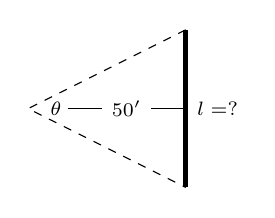
\begin{tikzpicture}
\draw [ultra thick] (1,-1) -- node [pos=.5,right] {\scriptsize $l=$?}(1,1);
\draw [dashed] (1,1) -- (-1,0) node [xshift=10pt] {\scriptsize $\theta$} -- (1,-1);
\draw (-.5,0) -- node [pos=.5,draw=white,fill=white] {\scriptsize $50'$} (1,0);
\end{tikzpicture}
\end{minipage}

\begin{enumerate}
\item		What is the measured length of the wall?
\item		What is the propagated error? 
\item		What is the percent error?
%\item		What is a key assumption about the location where the angle is measured? 
\end{enumerate}
}
{\begin{enumerate}
\item		298.9 feet
\item		$\pm 8.67$ ft
\item		$\pm 2.9$\%
%\item		Is is assumed that the location is halfway along the wall. 
\end{enumerate}
}

